\documentclass[10pt,]{beamer}
\hypersetup{pdfpagemode=FullScreen}

\usepackage{pgfpages}
\usepackage[style=authortitle,backend=bibtex]{biblatex}
\usepackage{animate}
% \bibliography{Bibliography}
\addbibresource{Bibliography.bib}

\mode<handout>{%
    \pgfpagesuselayout{4 on 1}[a4paper,landscape] 
    %\setbeameroption{show notes}
    \setbeamercolor{note page}{bg=white}
}

\usepackage[]{amsmath}
\usepackage{amsthm,amssymb,amsfonts}
\usepackage{graphicx,xfrac,mathrsfs,subcaption}
\usepackage{tikz,pgfplots}
\usepackage{tikzpagenodes}
\usepackage{multicol,multirow}
\usepackage{algorithm2e}
\usepackage{algorithmic}

\usetikzlibrary{positioning,automata}
\usetikzlibrary{matrix}
\usetikzlibrary{arrows,shapes}
\usetikzlibrary{trees}
\usetikzlibrary{backgrounds}
\usetikzlibrary{shapes.geometric}
\usetikzlibrary{calc,shapes.callouts,shapes.arrows}
\usetikzlibrary{graphs}
\usetikzlibrary{positioning, arrows}
\usetikzlibrary{fit}

\tikzset{onslide/.code args={<#1>#2}{%
  \only<#1>{\pgfkeysalso{#2}}
}}


%%%%%%%%%%%%%%%%%%%%%%%%%%%%
%%%%%%%%%%%%%%%%%%%%%%%%%%%%
%%%%% long and short versions
\newcommand{\extra}[1]{}
\newcommand{\short}[1]{#1}

% Custom colors
\definecolor{darkGreen}{HTML}{023618}
\definecolor{darkPurple}{HTML}{1C0221}
\definecolor{textGreen}{HTML}{628B48}

% Custom theorem styles
\makeatletter
\def\th@conjectureStyle{%
    \normalfont % body font
    \setbeamercolor{block title example}{bg=darkGreen,fg=white}
    \setbeamercolor{block body example}{bg=darkGreen!20,fg=black}
    \def\inserttheoremblockenv{exampleblock}
  }
\makeatother
\theoremstyle{conjectureStyle}
\newtheorem*{conjecture}{Conjecture}

\makeatletter
\def\th@notationStyle{%
    \normalfont % body font
    \setbeamercolor{block title example}{bg=darkPurple,fg=white}
    \setbeamercolor{block body example}{bg=darkPurple!20,fg=black}
    \def\inserttheoremblockenv{exampleblock}
  }
\makeatother
\theoremstyle{notationStyle}
\newtheorem*{notation}{Notation}

\usetheme{Boadilla}
\makeatother
\setbeamertemplate{footline}
{
	\leavevmode%
	\hbox{%
	\begin{beamercolorbox}[wd=.4\paperwidth,ht=2.25ex,dp=1ex,center]{author in head/foot}%
		\usebeamerfont{author in head/foot}\insertshortauthor
	\end{beamercolorbox}%
	\begin{beamercolorbox}[wd=.6\paperwidth,ht=2.25ex,dp=1ex,center]{title in head/foot}%
		\usebeamerfont{title in head/foot}\insertshorttitle\hspace*{3em}
		\insertframenumber{} / \inserttotalframenumber\hspace*{1ex}
	\end{beamercolorbox}}%
	\vskip0pt%
}
\makeatletter

\setbeamertemplate{navigation symbols}{}
\title[HK-property | Perfect Binary Trees]{Exploring perfect binary trees with relation to the HK-property}
\subtitle{MXML Presentation} %This is where you can specify the conference name or presentation venue
\author[A.M, M.N.S]{Atishaya Maharjan \\ Mahsa N. Shirazi}
\date{\today}

\begin{document}
\parskip = \baselineskip

\begin{frame} %Title page
    \titlepage
\end{frame}

\begin{frame}{Outline}
    \tableofcontents
\end{frame}

\begin{frame}
    \frametitle{Introduction}
    \begin{itemize}
        \item Providing an overview of the Erdős-Ko-Rado (EKR) theorem and its relevance to intersecting families of sets.
        \item Introducing perfect binary trees and their relation to the HK-property.
        \item Objectives of this presentation:
              \begin{itemize}
                  \item Exploring properties of perfect binary trees.
                  \item Discussing the HK-property.
                  \item Investigating potential connections between perfect binary trees and the HK-property.
              \end{itemize}
    \end{itemize}
\end{frame}

\begin{frame}\frametitle{EKR Theorem}
    \begin{itemize}
        \item \footcite{Erds1961INTERSECTIONTF} The Erdős-Ko-Rado (EKR) theorem, named after mathematicians Paul Erdős, Chao Ko, and Richard Rado, is a fundamental result in extremal set theory.
        \item The theorem deals with intersecting families of sets, which are collections of sets that share a common non-empty intersection.
        \item  Specifically, the EKR theorem provides conditions under which the size of the largest intersecting family of sets can be determined.
        \item \footcite{MR0892525} This result has applications in combinatorics, graph theory, probability and other areas of statistics and mathematics.
    \end{itemize}
\end{frame}

\section{EKR Theorem}
\begin{frame}\frametitle{EKR Theorem}
    \begin{definition}[Intersecting family]
        A family of subsets $\mathcal{F}$ of some set is \textbf{intersecting} if any two members of $\mathcal{F}$ have a non-empty intersection.
    \end{definition}
    \begin{itemize}
        \item The \textbf{Erd\H{o}s-Ko-Rado} theorem limits the number of sets in an intersecting family.
    \end{itemize}
    \begin{theorem}[EKR Theorem]
        \footcite{Erds1961INTERSECTIONTF} If $\mathcal{F}$ is an intersecting family of $k$-subsets of an $n$-set (cardinality of the set is $n$), then
        \begin{itemize}
            \item $|\mathcal{F}| \leq \binom{n - 1}{k - 1}$
            \item If equality holds, $\mathcal{F}$ consists of the $k$-subsets that contain $i$, for some $i$ in the $n$-set.
        \end{itemize}
    \end{theorem}
\end{frame}

\section{HK-property}
\begin{frame}\frametitle{HK-property}
    \begin{definition}[Cocliques]
        \begin{itemize}
            \item A \textbf{coclique} in a graph is a set of vertices such that no two vertices in the set are adjacent.
            \item The maximum size of a coclique in a graph is called the \textbf{indepdence number} of the graph. For a graph $G$, it is denoted by $\alpha(G)$.
        \end{itemize}
    \end{definition}

    \begin{definition}[Stars and Stars Center]
        \begin{itemize}
            \item Let $G = (V, E)$ be a graph, and $v \in V$. The set of all cocliques of $G$ of cardinality $n$ is denoted as $\mathcal{I}^n_T$.
            \item For $v \in V$, the family $\mathcal{I}^n_G(v) = \{A \in \mathcal{I}^n_G : v \in A\}$ is called a \textbf{star} of $\mathcal{I}^n_G$ and $v$ is called its \textbf{start center}.
        \end{itemize}
    \end{definition}

    \begin{definition}[k-EKR graph]
        A graph is said to be $k$-EKR if for any family of cocliques $\mathcal{F} \in \mathcal{I}^n_G$ with the intersection of any two sets in $\mathcal{F}$ being non-empty, there is a vertex $v \in V$ such that $|\mathcal{F}| \leq \mathcal{I}^n_G(v)$.
    \end{definition}
\end{frame}

\begin{frame}\frametitle{HK-property}
    Studying the EKR theorem, \footcite{HOLROYD2005165} Holroyd and Talbot made the following two conjectures:
    \begin{conjecture}[k-EKR Conjecture]
        Let $G$ be a graph, and let $\mu(G)$ be the size of its smallest maximal coclique. Then $G$ is $k$-EKR for every $1 \leq k \leq \frac{\mu(G)}{2}$.
    \end{conjecture}
    \begin{conjecture}[HK-Property]
        For any $k \geq 1$ and any tree $T$, there exists a leaf $l$ of $T$ such that $|\mathcal{I}^k_T(v)| \leq |\mathcal{I}^k_T(l)|$ for each $v \in V(T)$.
    \end{conjecture}
\end{frame}

\begin{frame}\frametitle{HK-property}
    \begin{itemize}
        \item The HK-property was proven for $k \leq 4$, but the conjecture was shown to be false.\footcite{MR2523796} \footcite{MR3612439} \footcite{MR3271819}
    \end{itemize}

    \begin{figure}
        \centering
        \begin{tikzpicture}[scale=0.7,level distance=2cm,
                level 1/.style={sibling distance=8cm},
                level 2/.style={sibling distance=4cm},
                level 3/.style={sibling distance=2cm},
                every node/.style={circle, draw, fill=white, minimum size=1.75em},]
            \node (v11) {$v_0$}
            child {node (v21) {$v_1$}
                    child {node  {}
                            child {node {}}
                        }
                    child {node (v32) {}
                            child {node {}}
                        }
                }
            child {node (v22) {$v_2$}
                    child {node (v33) {}
                            child {node {}}
                        }
                    child {node (v34) {}
                            child {node {}}
                        }
                };
        \end{tikzpicture}
        \caption*{Figure 1: The largest k-star for $k \geq 5$ is centered at $v_0$}
    \end{figure}
\end{frame}

\begin{frame}\frametitle{Some graphs that DO satisfy the HK-property \footcite{MR2763040}}
    \begin{itemize}
        \item \textbf{Caterpillars:} A tree such that when you remove the leaves and incident edges, you get a path.
        \item \textbf{Lobsters*:} A tree such that when you remove the leaves and incident edges, you get a caterpillar.
        \item \textbf{Spiders:} A tree with exactly one vertex of degree greater than 2.
    \end{itemize}

    *Note: The graph shown in Figure 1 is a lobster. As such, it does not strictly satisfy the HK-property. Instead, the largest stars are centered at the vertices of degrees 1 or 2.
\end{frame}

\section{Perfect Binary Trees}
\begin{frame}\frametitle{Perfect Binary Tree}
    \begin{definition}[Depth of a vertex]
        For a tree $T = (V, E)$ with a root vertex $r \in V$, the \textbf{depth} of a vertex $v \in V$ is defined as the length of the path from the $r$ to $v$.
    \end{definition}
    \begin{definition}[Binary Tree]
        A \textbf{binary tree} is a tree in which each vertex has at most two children, referred to as the left child and the right child.
    \end{definition}
    \begin{definition}[Perfect Binary Tree]
        A \textbf{perfect binary tree} is a binary tree in which all the internal nodes have exactly two children and all the leaves are at the same depth.
    \end{definition}
\end{frame}



\section{Does a perfect binary tree satisfy the HK property?}
\begin{frame}\frametitle{Does a perfect binary tree satisfy the HK property?}
    \begin{itemize}
        \setlength\itemsep{2em}
        \item Probably.
        \item The lobster almost satisfies the HK property and the perfect binary tree has a close relation to the lobster.
        \item In addition, the perfect binary tree is very symmetric and has a lot of structure that we can maniputlate.
    \end{itemize}
\end{frame}

\section{Idea 1}
\begin{frame}\frametitle{Idea 1: Expand the definition of the flip function to relate it to the perfect binary trees}
    \begin{itemize}
        \item Estrugo and Pastine\footcite{MR2763040} proved the HK-property holds for caterpillars and partially lobsters by utilizing a `flip' function alongside an `escape-path' property.

        \item Why not expand the definition of the flip function to fit it to perfect binary trees?
    \end{itemize}
\end{frame}


\begin{frame}\frametitle{Idea 1: Expand the definition of the flip function to relate it to the perfect binary trees}
    \begin{definition}[Escape Paths]
        \footcite{MR2763040}Let $G = (V, E)$ be a graph and $P = v_1v_2, \ldots , v_n$ a path of length $n$ such that $P \subset G$. We say that $P$ is an \textbf{escape path} from $v_1$ to $v_n$ if $deg(v_n) = 1$ and $deg(v_i) = 2$ for every $2 \leq i \leq n - 2$. If this is the case, we say that $v_1$ has an escape path to $v_n$.
    \end{definition}

    \begin{definition}[Flip function]
        Let $G = (V, E)$ be a graph and $P = v_1v_2, \ldots, v_n$ be an escape path from $v_1$ to $v_n$ in $G$. Then the flip of $P$ in $G$, flip$_P$ : $V \rightarrow V$, is the function defined as follows:
        \begin{align*}
            \text{flip}_P(v) = \begin{cases}
                                   v             & \text{if } v \not\in V(P)   \\
                                   v_{n + 1 - i} & \text{if } v = v_i \in V(P)
                               \end{cases}
        \end{align*}
    \end{definition}
\end{frame}

\begin{frame}\frametitle{Idea 1: Expand the definition of the flip function to relate it to the perfect binary trees}
    We need to address the following questions:
    \begin{itemize}
        \item How do we enumerate our vertices in the perfect binary tree so that we can use it in the flip function?
        \item How do we define a flip function so that it works for any vertex in the perfect binary tree?
        \item How do we define the escape paths in the perfect binary tree?
    \end{itemize}
\end{frame}

\begin{frame}\frametitle{Idea 1: Expand the definition of the flip function to relate it to the perfect binary trees}
    \begin{notation}
        Let $\mathcal{V}_k \in V(T)$ be the set of vertices of depth $k$. We call $\mathcal{V}_k$ as the depth vertex set of depth $k$. Index all vertices in $\mathcal{V}_k$ from left to right as $v_{k, i}$, where $k$ is the depth of the vertex and $i$ is the index of the vertex in $\mathcal{V}_k$ such that $1 \leq i \leq 2^{k - 1}$.
    \end{notation}
    \begin{figure}
        \centering
        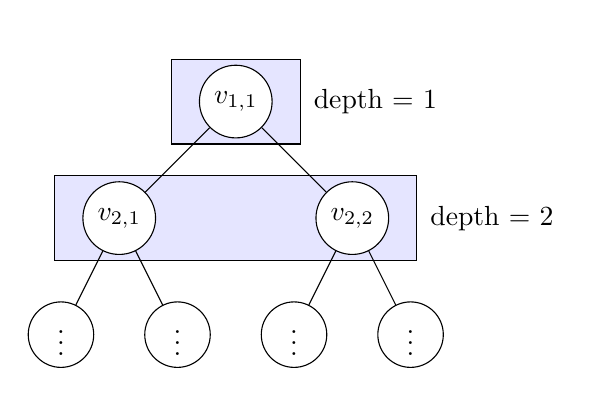
\begin{tikzpicture}[scale=0.37,level distance=4cm,
                level 1/.style={sibling distance=8cm},
                level 2/.style={sibling distance=4cm},
                level 3/.style={sibling distance=2cm},
                every node/.style={circle, draw, fill=white}]
            \node (v11) {$v_{1,1}$}
            child {node (v21) {$v_{2,1}$}
                    child {node {$\vdots$}}
                    child {node {$\vdots$}}
                }
            child {node (v22) {$v_{2,2}$}
                    child {node {$\vdots$}}
                    child {node {$\vdots$}}
                };

            \begin{scope}[on background layer]
                \node[draw,rectangle,fit=(v11),inner xsep=10pt, inner ysep=2pt, fill=blue!10, label=right:{depth = 1}] {};
                \node[draw,rectangle,fit=(v21) (v22),inner xsep=10pt, inner ysep=2pt, fill=blue!10, label=right:{depth = 2}] {};
            \end{scope}
        \end{tikzpicture}
    \end{figure}
\end{frame}

\begin{frame}\frametitle{Idea 1: Expand the definition of the flip function to relate it to the perfect binary trees}
    To show that our flip function can work on any vertex, we approach it by defining a helper flip function on every depth vertex set.

    \begin{definition}[Flip Function on Depth Vertex Set]
        Let $T$ be a perfect binary tree and $\mathcal{V}_k$ be the depth vertex set of depth $k$. Then, the flip of $\mathcal{V}_k$ in $T$, denoted by $flip_\mathcal{K}: \mathcal{V}_k(G) \rightarrow \mathcal{V}_k(G)$, is the function defined as follows:

        \begin{equation*}
            flip_\mathcal{K}(v_{(k, i)}) = \begin{cases}
                v_{(k, 2^{k-1} + 1 - i)}  & \text{if } N_T(v_{(k, 2^{k - 1} + 1 - i)}) \not\subseteq \mathcal{I}_T(v_{(k, 2^{k - 1} + 1 - i)}) \\
                v_{(k, 2^{k-1} + 1 - i)}, & \text{if } N_T(v_{(k, 2^{k - 1} + 1 - i)}) \subseteq \mathcal{I}_T(v_{(k, 2^{k - 1} + 1 - i)})     \\
                flip_N(v_{(k, i)}),       & \text{if } N_T(v_{(k, 2^{k - 1} + 1 - i)}) \subseteq \mathcal{I}_T(v_{(k, 2^{k - 1} + 1 - i)})
            \end{cases}
        \end{equation*}

        \text{where, $flip_N$ is defined as:}
        \begin{equation*}
            flip_N(v_{(k, i)}) =  flip_\mathcal{K}(u), \text{ for all } u \in N_T(v_{(k, i)})
        \end{equation*}
    \end{definition}
\end{frame}


\begin{frame}\frametitle{Idea 1: Expand the definition of the flip function to relate it to the perfect binary trees}
    Then utilizing the flip function on the depth vertex set, we tried to define the flip function diagonally on the perfect binary tree.

    Our approach is as follows:

    \begin{itemize}
        \item Pick any leaf $\ell$.
        \item Utilize the flip$_\mathcal{K}$ function on the depth vertex set of $\ell$ to flip it with either $\ell_{(k, 2^{k - 1} + 1)}$ or $\ell_{(k, 0)}$ (The leaves at the very extremes).
        \item Take the path $P$ from the root to $l$.
        \item Apply a `diagonal' flip function on $P$. (Note: This is still a work in progress).
    \end{itemize}
\end{frame}

\begin{frame}\frametitle{Idea 1: Expand the definition of the flip function to relate it to the perfect binary trees}
    We have now addressed 2 of the 3 questions:
    \begin{itemize}
        \item \textcolor{textGreen}{How do we enumerate our vertices in the perfect binary tree so that we can use it in the flip function?}
        \item \textcolor{textGreen}{How do we define a flip function so that it works for any vertex in the perfect binary tree?}
        \item \textcolor{red}{How do we define the escape paths in the perfect binary tree?}
    \end{itemize}
\end{frame}

\begin{frame}\frametitle{Idea 1: Expand the definition of the flip function to relate it to the perfect binary trees}
    Unfortunately, we were unable to expand the definition of the escape path to the perfect binary tree. This is because it does not satisfy the core idea that we can generate a single path aside from the 2 vertices that we seek to flip. This is primarily due to the fact that all internal vertices (Excluding the root) have degree 3.
\end{frame}

\section{Idea 2}
\begin{frame}\frametitle{Idea 2: Use an enumeration approach with computer algorithms to verify the results}
    \begin{algorithm}[H]
        \KwData{$n \geq 0$, where $n$ is the depth of the perfect binary tree}
        \KwResult{A perfect binary tree graph's leaves}

        \SetKwFunction{FMain}{perfect\_binary\_tree\_generator}

        \SetKwProg{Fn}{Function}{:}{}
        \Fn{\FMain{$n$}}{
            $num\_vertices \gets 2^{n + 1} - 1$\;
            $leaves \gets []$\;
            $last\_row\_start \gets floor(num\_vertices / 2)$\;
            \For{$vertex$ in range($last\_row\_start$, $num\_vertices$)}{
                $leaves$.append($vertex$)\;
            }
            \Return{$leaves$}
        }
    \end{algorithm}
\end{frame}

\begin{frame}\frametitle{Idea 2: Use an enumeration approach with computer algorithms to verify the results}
    The algorithm will generate a perfect binary tree of this form:
    \begin{figure}[hbt!]
        \centering

        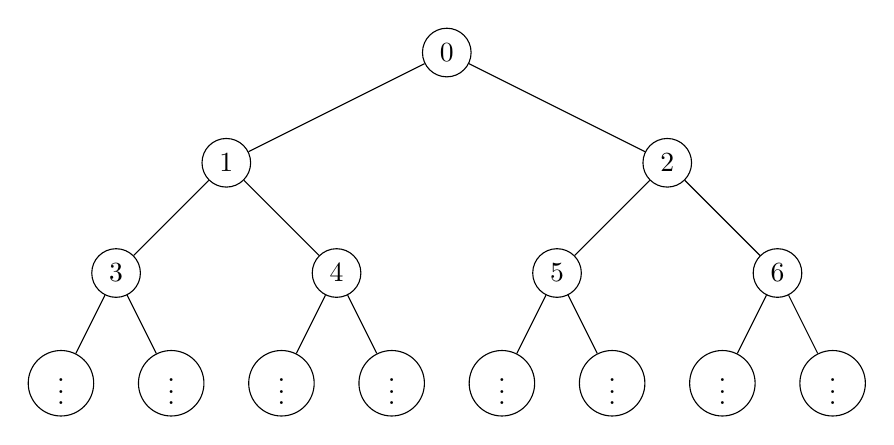
\begin{tikzpicture}[scale=0.7,level distance=2cm,
                level 1/.style={sibling distance=8cm},
                level 2/.style={sibling distance=4cm},
                level 3/.style={sibling distance=2cm},
                every node/.style={circle, draw, fill=white}]
            \node (0) {$0$}
            child {node (1) {$1$}
                    child {node (3) {$3$}
                            child {node {$\vdots$}}
                            child {node {$\vdots$}}
                        }
                    child {node (4) {$4$}
                            child {node {$\vdots$}}
                            child {node {$\vdots$}}
                        }
                }
            child {node (2) {$2$}
                    child {node (5) {$5$}
                            child {node {$\vdots$}}
                            child {node {$\vdots$}}
                        }
                    child {node (6) {$6$}
                            child {node {$\vdots$}}
                            child {node {$\vdots$}}
                        }
                };
        \end{tikzpicture}
    \end{figure}
\end{frame}

\section{Idea 2}
\begin{frame}\frametitle{Idea 2: Use an enumeration approach with computer algorithms to verify the results}
    We then use the algorithm from ~\cite{Niskanen2003CliquerUG} to generate a coclique of maximum cardinality for our perfect binary tree.

    \begin{algorithm}[H]
        % \caption{Maximum Indpendent Set Algorithm}\label{alg:max-independent-set}
        \KwData{A perfect binary tree graph $T$}
        \KwResult{A maximum coclique of $T$}

        \SetKwFunction{FMain}{maximum\_coclique}

        \SetKwProg{Fn}{Function}{:}{}
        \Fn{\FMain{$T$}}{
            $cliquer \gets Cliquer(T)$\;
            \Return{$cliquer$.get\_maximum\_coclique()}
        }
    \end{algorithm}
\end{frame}

\begin{frame}\frametitle{Idea 2: Use an enumeration approach with computer algorithms to verify the results}
    \begin{algorithm}[H]
        \KwData{A perfect binary tree graph $T$}
        \KwResult{All cocliques of $T$}

        \SetKwFunction{FMain}{enumerate\_cocliques}

        \SetKwProg{Fn}{Function}{:}{}
        \Fn{\FMain{$T$}}{
            $cocliques \gets []$\;
            $cocliques$.append($\emptyset$)\;
            \For{$vertex$ in $T$}{
                $new\_cocliques \gets []$\;
                \For{$coclique$ in $cocliques$}{
                    \For{$neighbor$ in $vertex.neighbors$}{
                        \If{$neighbor \not\in coclique$}{
                            $new\_coclique \gets coclique \cup \{neighbor\}$\;
                            $new\_cocliques$.append($new\_coclique$)\;
                        }
                    }
                }
                $cocliques \gets new\_cocliques$\;
            }
            \Return{$cocliques$}
        }
    \end{algorithm}
\end{frame}

\begin{frame}\frametitle{Idea 2: Use an enumeration approach with computer algorithms to verify the results}
    \begin{itemize}
        \item We can then use the results from the algorithm to verify the HK-property for perfect binary trees.
        \item Do note that the algorithm is a brute-force approach and is not efficient for large trees. Hence, in the future we plan to optimize the algorithm.
    \end{itemize}
\end{frame}


\begin{frame}\frametitle{Idea 2: Use an enumeration approach with computer algorithms to verify the results}
    This is the data for a perfect binary tree of depth 5.
    \centering
    \animategraphics[loop,width=8cm]{21}{size_}{1}{21}
\end{frame}

\begin{frame}\frametitle{Idea 2: Use an enumeration approach with computer algorithms to verify the results}
    \begin{itemize}
        \item The results do indeed verify that the HK-property holds for perfect binary trees of depth 5. With the pattern, we do believe it holds for any depth perfect binary tree.
        \item However, it is clearly still not a proof.
    \end{itemize}
\end{frame}

\begin{frame}\frametitle{Idea 3: An inductive proof}
    \begin{conjecture}[Maximum coclique size of perfect binary trees contains all the leaves]
        For a given perfect binary tree $T$ of depth $d$, the
    \end{conjecture}
\end{frame}



%%%%%%%%%%%%%%%%%%%%%%%%%%%%%%%%%%%%%%%%%%%%%%%%%%%%%%%%%%%%%%%%%%%%%%
%%%%%%%%%%%%%%%%%%%%%%%%%%%%%%%%%%%%%%%%%%%%%%%%%%%%%%%%%%%%%%%%%%%%%%  
%%%%%%%%%%%%%%%%%%%%%%%%%%%%%%%%%%%%%%%%%%%%%%%%%%%%%%%%%%%%%%%%%%%%%%
\begin{frame}\frametitle{Thank You!}
    \framesubtitle{Summary}
    \begin{itemize}
        \item We explored the Erdős-Ko-Rado theorem and its relevance to intersecting families of sets.
        \item Introduced perfect binary trees and their relation to the HK-property.
        \item Discussed the HK-property and its relevance to intersecting families of sets.
        \item Demonstrated the use of computer algorithms to verify the HK-property for perfect binary trees of depth 5.
        \item Presented three ideas to investigate the HK-property for perfect binary trees.
    \end{itemize}
\end{frame}
%%%%%%%%%%%%%%%%%%%%%%%%%%%%%%%%%%%%%%%%%%%%%%%%%%%%%%%%%%%%%%%%%%%%%%
%%%%%%%%%%%%%%%%%%%%%%%%%%%%%%%%%%%%%%%%%%%%%%%%%%%%%%%%%%%%%%%%%%%%%%  
%%%%%%%%%%%%%%%%%%%%%%%%%%%%%%%%%%%%%%%%%%%%%%%%%%%%%%%%%%%%%%%%%%%%%%

\end{document}